\documentclass[]{standalone}
\usepackage[utf8]{inputenc}
\usepackage[american]{circuitikz}
\usetikzlibrary{arrows,shapes,calc,positioning}

\usepackage{graphicx}


\begin{document}
 
  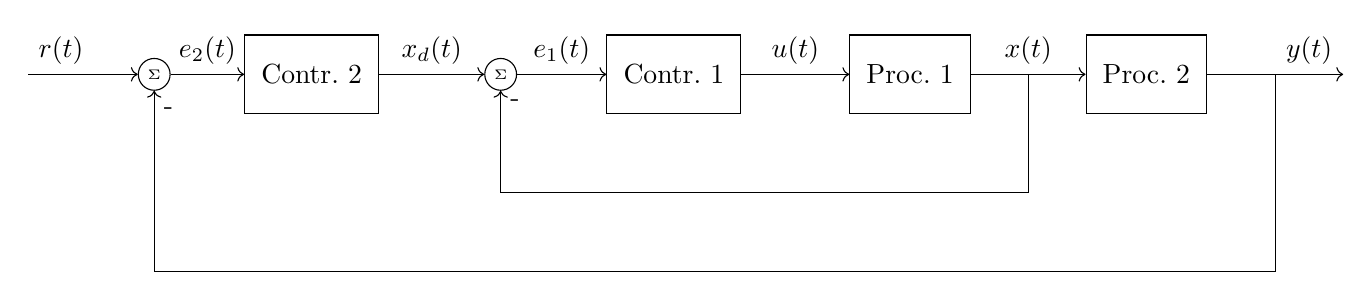
\begin{tikzpicture}[node distance=22mm, block/.style={rectangle, draw, minimum width=15mm, minimum height=10mm, inner sep=6pt}, sumnode/.style={circle, draw, inner sep=2pt}]
    
    \node[coordinate] (input) {};
    \node[sumnode, right of=input, node distance=16mm] (sum2) {\tiny $\Sigma$};
    \node[block, right of=sum2, node distance=20mm] (controller2)  {Contr.~2};
    \node[sumnode, right of=controller2, node distance=24mm] (sum) {\tiny $\Sigma$};
    \node[block, right of=sum, node distance=22mm] (controller1)  {Contr.~1};
    \node[block, right of=controller1, node distance=30mm] (plant1)  {Proc.~1};
    \node[block, right of=plant1, node distance=30mm] (plant2)  {Proc.~2};
    \node[coordinate, right of=plant2, node distance=25mm] (output) {};

    \draw[->] (input) -- node[above, pos=0.3] {$r(t)$} (sum2);
    \draw[->] (sum2) -- node[above] {$e_2(t)$} (controller2);
    \draw[->] (sum) -- node[above] {$e_1(t)$} (controller1);
    \draw[->] (controller2) -- node[above] {$x_{d}(t)$} (sum);
    \draw[->] (controller1) -- node[above] {$u(t)$} (plant1);
    \draw[->] (plant1) -- node[above] {$x(t)$} node[coordinate] (m1) {} (plant2);
    \draw[->] (m1) -- ++(0,-15mm) -| node[right, pos=0.95] {-} (sum);
    \draw[->] (plant2) -- node[coordinate,] (m2) {} node[above, near end] {$y(t)$} (output);
    \draw[->] (m2) -- ++(0,-25mm) -| node[right, pos=0.95] {-} (sum2);

    %\draw[red] (sum) ++(-4mm,-20mm) rectangle ++(95mm, 30mm);
    %\node[red] at (140mm,-15mm) {\large $G_2(s)$};
  \end{tikzpicture}

  
\end{document}
